%************************************************
\chapter{Evolution of protein-coding genes in gorilla and the African apes}
\label{ch_gorilla}
%************************************************

\section{Introduction}

The search for what defines us as humans is a recurring theme in
biology. The field of molecular evolution has deep roots in the use of
molecules to compare humans with our closest relatives, gorilla and
chimpanzee: in the 1960s Zuckerkandl and Pauling's applied their
molecular clock hypothesis to estimate the gorilla-human divergence
time, and \citeauthor{King1975}'s infamous 1975 paper ``Evolution at
Two Levels in Humans and Chimpanzees'' proposed that changes to the
expression of genes, rather than changes within protein-coding regions
themselves, may be primarily responsible for the observed anatomical
and behavioral differences between humans and chimpanzees
\citep{King1975}. Figure \ref{fig_king_wilson} shows the schematic
used by \citeauthor{King1975} to illustrate the proposed disconnect
between organismal and molecular rates of evolution: whereas human
shows signs of having changed more from the human-chimpanzee ancestor
in terms of behavior and anatomy, more equal rates of molecular
evolution were observed.

\begin{figure}
\centering
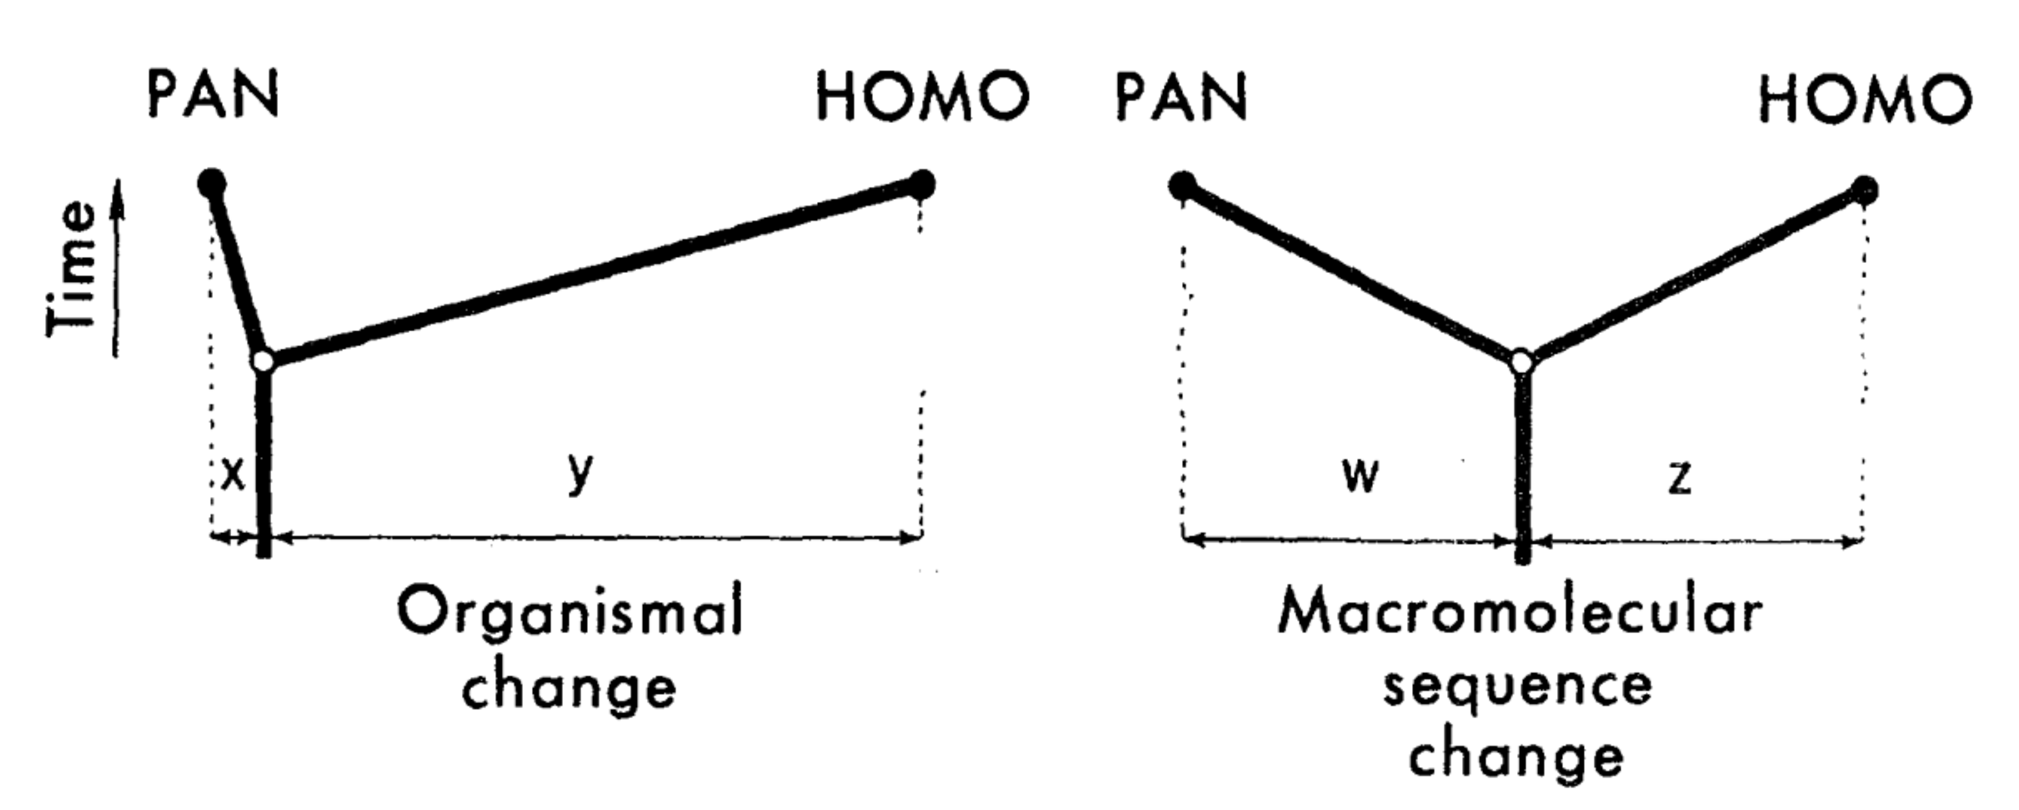
\includegraphics[scale=0.35]{Figs/king_wilson.pdf}
\caption{Schematic diagram of the rates of organismal and molecular
  change in human (Homo) and chimpanzee (Pan). Figure taken from
  \citet{King1975}.}
\label{fig_king_wilson}
\end{figure}

Continued genetic, anatomical and \emph{in situ} study of primates has
somewhat tempered the imbalance in the ``organismal'' rates of human
and chimpanzee evolution as drawn by King and Wilson: the evolution of
human form does not appear to be exceptional within the context of
other mammalian and primate species \citep{Carroll2003}, and humans
variously share and differ in many behavioral and sexual
characteristics with chimpanzee and gorilla
\citep{Harcourt1980,Goodall1986,Vigilant2004}. On the molecular level,
however, few plausible connections between human-specific phenotypes
and molecular changes have been found, lending support to King and
Wilson's 30-year old prediction
\citep{Clark2003,Sequencing2005a,Bradley2008}. In the first comparison
of the human and chimpanzee genomes, \citet{Sequencing2005a} wrote
that ``We thus find minimal evidence of acceleration unique to either
the human or chimpanzee lineage across broad functional categories.''
Still, these general findings do not preclude the possibility of
\emph{some} amount of protein-coding change playing a role in the
differences between humans and our close relatives. Accordingly,
studies of protein-coding evolution in humans and our close relatives
have provided insight into the evolution of the great apes as a whole,
identifying patterns of adaptive evolution or relaxed constraint in
genes related to sound perception \citep{Clark2003}, coloration
\citep{Mundy2007}, language \citep{Enard2002} and brain size
\citep{Montgomery2011}. Adaptive evolution in genes related to sperm
production \citep{Clark2005} and immune defense \citep{Sawyer2005a}
has also repeatedly been found in primates, though these patterns of
selective pressures appear to be shared throughout the mammalian
clade, as evinced in Chapter \ref{ch_mammals2}.

Within this context, the recent sequencing of a western lowland
gorilla genome provided an opportunity to further examine patterns of
molecular evolution within human and our closest living relatives,
even if the power to detect lineage-specific adaptive events (or the
actual presence of such events) was likely to be limited. Previous
phylogenetic estimates indicate that the \ac{hcg} common ancestor
lived 6-10 \ac{myr} ago, with humans and chimpanzees diverging a few
\ac{myr} after that \citep{Bradley2008}. The inclusion of gorilla
within a comparative analysis would thus provide 6-10 \ac{myr} of
additional branch length to the primate tree in addition to allowing
the distinction between substitutions along the \ac{hcg} and the
\ac{hc} ancestral branches of the phylogenetic tree. With gorilla,
potential differences in the molecular evolution of our distant (e.g.,
\ac{hcg}) and more recent (e.g., \ac{hc}) great ape ancestors could be
investigated. Furthermore, analysis of the terminal branch of gorilla
could provide additional information regarding the constancy or
variability of evolutionary rates in the recent evolution of the
\ac{aga} (e.g., human, chimpanzee and gorilla). Previous analyses have
estimated a greater \ac{ne} in chimpanzee compared to human
\citep{Sequencing2005a,Siepel2009a}, and somewhat surprisingly, one
study identified more lineage-specific \acp{psg} in chimpanzee than in
human (\citet{Bakewell2007}, but see \citet{Mallick2009} for evidence
of false positives in these results). Gorilla, representing a third
independent \ac{aga} lineage with a slightly longer branch length than
human and chimpanzee, will provide an important additional data point
in this regard.

In collaboration with Stephen Montgomery and Nick Mundy from the
Zoology department of Cambridge University, I performed an analysis of
the evolution of protein-coding genes in gorilla and the \ac{aga}. The
analysis was jointly designed by Stephen, Nick and myself; all data
collection, calculations and statistical analyses were performed by
me; and results were interpreted by us and other members of the
gorilla analysis consortium. As with the analysis for the \ac{mgp}, a
summary of our main findings was contributed to the manuscript
describing the gorilla genome, which is currently undergoing peer
review. The description of the methods and results presented here is
similar to the text included in the submitted manuscript and
supplementary documents.

The main goal of the analysis was to use codon models of evolution to
identify genes with accelerated \nsyn substitution rates in the
terminal and ancestral branches of the \ac{aga}. To do this, I
collected a highly filtered set of coding alignments in six primate
species (the African great apes plus orangutan, rhesus macaque, and
marmoset) and used a series of \acp{lrt} based on the branch models
implemented in \acp{paml} to identify accelerated genes along branches
of the primate phylogeny. Within the wider context of the gorilla
genome analysis, which included an investigation of \ac{ils} in coding
and non-coding regions, a secondary goal of this study was to identify
patterns of \ac{ils} within and near protein-coding genes. A third
goal was to use the set of genome-wide coding alignments to estimate
lineage-specific average \dnds ratios. Through the connection between
\ac{ne} and \dnds, these results could be used to place gorilla and
the ancestral \ac{aga} branches within the wider context of changing primate population sizes through time \citep{Sequencing2005a}.

\section{Data collection and quality control}
\subsection{Primate one-to-one orthologous genes}

All orthologous gene sets, gene trees, and sequence alignments were
collected from Ensembl Compara release 60 using the Ensembl Perl API
\citep{Vilella2009,Flicek2011}. I first identified the set of genes
sharing one-to-one orthology among all six primates by collecting
homology annotations from the \ens \cmp database: for each human
protein-coding gene, the orthology status for each non-human species
was assigned to different categories based on the number of homologous
genes and the type of homology as annotated by \ens. Homologs were
classified as either one-to-one (e.g., one homolog available and
either an ``ortholog\_one2one'' or ``apparent\_ortholog\_one2one''
homology type), deleted (e.g., no homolog available), duplicated
(e.g., multiple homologs available), or human duplication (e.g., one
homolog available but containing an ``ortholog\_one2many'' annotation,
indicating that there are multiple human homologs for that single
non-human homolog). From an initial set of 20,746 human protein-coding
genes, this procedure identified 12,652 genes with 6-way 1-to-1
orthology; 4,809 genes with primate deletions; 1,171 genes with
primate duplications; 308 genes with human-specific duplications; and
1,806 genes with mixed patterns of duplication and deletion.

\begin{figure}
\centering
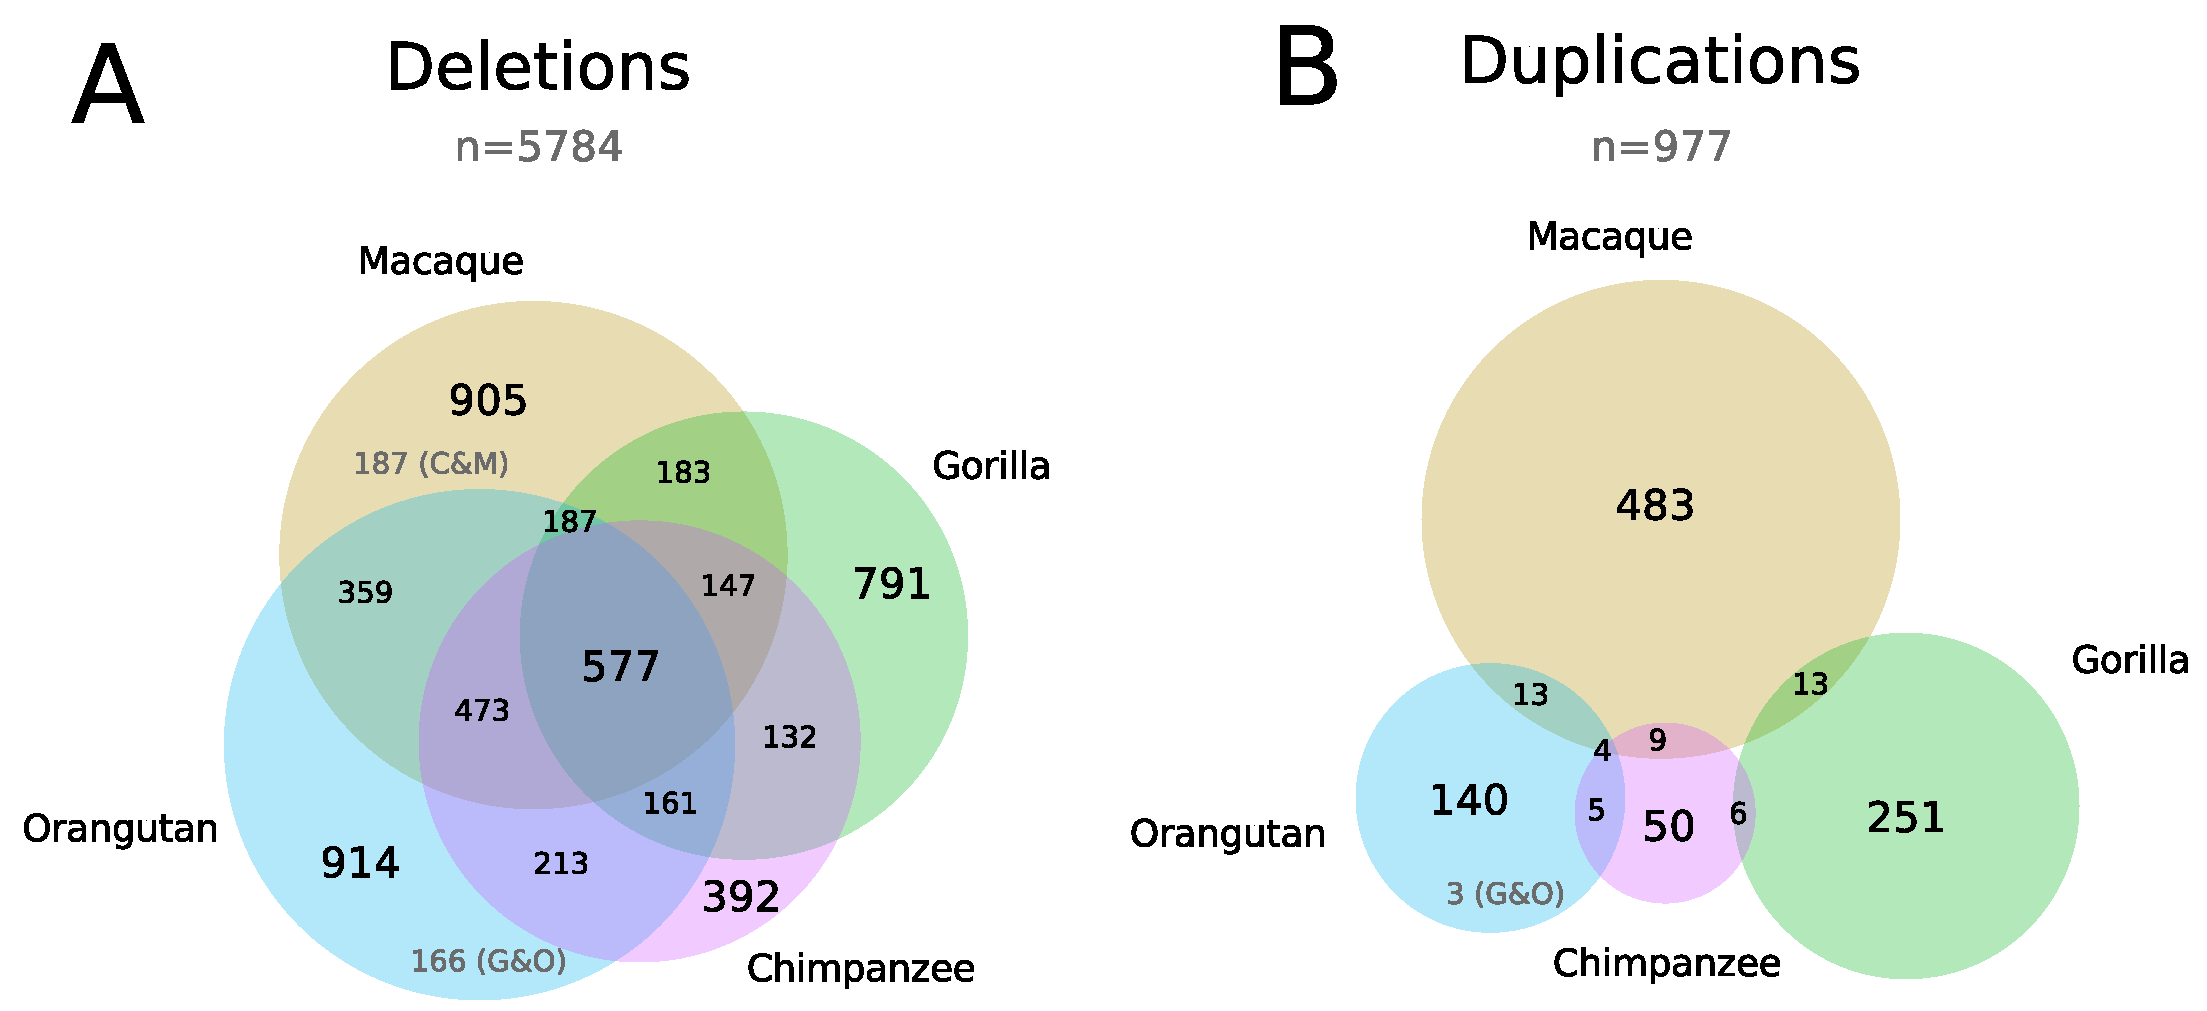
\includegraphics[scale=0.4]{Figs/gorilla_dup_dels.pdf}
\caption{Venn diagrams of shared and unique (A) deletions and (B)
  duplications in non-human primates relative to the set of human
  genes.}
\label{fig_gorilla_dup_dels}
\end{figure}

Figure \ref{fig_gorilla_dup_dels} shows two Venn diagrams of shared
gene deletions and duplications in chimpanzee, gorilla, orangutan and
macaque relative to the human set of protein-coding genes. The \emph{a
  priori} expectation, assuming somewhat random ongoing process of
gene duplication and deletion, was that species most closely related
to human would contain fewer deletions and duplications relative to
the human gene set, with increasingly distant species having greater
numbers. Ignoring the overlap, a comparison of the size of each
species' circle in Figure \ref{fig_gorilla_dup_dels}A showed this to
be the case: 2,279 deletions were found for chimpanzee, 2,344 for
gorilla, 3,050 for orangutan, and 3,015 for macaque (marmoset, not
shown, had 3,215 deletions). The counts of duplications showed a
similar pattern, except for a notable excess of gorilla duplications:
gorilla had 273 duplications relative to human, compared to 74 in
chimpanzee, 165 in orangutan, 522 in macaque, and 722 in marmoset. The
excess of duplications in gorilla appeared to be anomalous, and is
expected to decrease in future refined versions of the gene annotation
set.

The amount of overlap between species in the Venn diagrams of Figure
\ref{fig_gorilla_dup_dels} shows how often deletions and duplications
relative to human are shared between different primate
species. Interestingly, deletions appeared to be more often shared
between two or more species than duplications, suggesting that certain
genes may be more prone to independent deletion events than
duplication events. It should be stressed, however, that this analysis
and view of gene duplications and deletions was not intended to
rigorously identify gene duplication and deletion events in
primates. A more appropriate approach would be to explicitly place
duplication and deletion events along the primate phylogeny using one
or multiple mammalian outgroups, but these comparisons were made
mostly to gain an understanding of whether gene deletions or
duplications were more responsible for genes which did not have
one-to-one orthology within \ac{aga}.

\begin{figure}
\centering
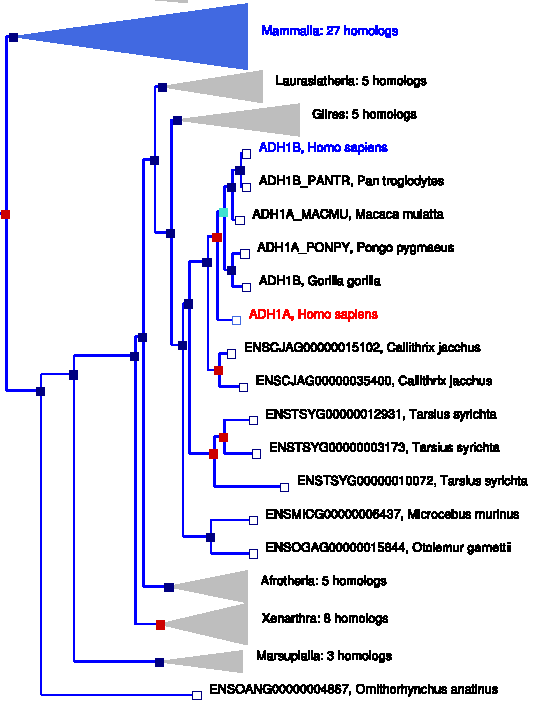
\includegraphics[scale=0.9]{Figs/adh1a.pdf}
\caption{Part of the inferred gene tree relating the human gene
  \gene{ADH1A} and its homologs. \gene{ADH1A} is highlighted in red
  and the human gene \gene{ADH1B} is highlighted in blue. The gene
  tree data were taken from \ens release 60.}
\label{fig_adh1a}
\end{figure}

Many of the shared deletions in Figure \ref{fig_gorilla_dup_dels} were
likely the result of recent human duplications where the homology to
other primate genes was not detected, either due to incorrect
assembly, missing primate gene annotations or the conservative rules
used by \ens to assign orthology relationships based on gene trees
\citep{Vilella2009}. An example is the gene \gene{ADH1A}: although the
homology annotations indicated the gene as lacking a homolog in all 5
of the primates included here, a detailed analysis of \gene{ADH} gene
family evolution identified clear one-to-one orthology between
\gene{ADH1A} genes within primates \citep{Oota2007}. The authors
showed that the cluster of \gene{ADH} genes likely arose through
mammalian-specific and primate-specific duplication events in
chromosome 4, raising the possibility that these duplicated genomic
segments could have been falsely collapsed into a single assembled
sequence in non-human assemblies. The \cmp gene tree for \gene{ADH1A},
pictured in Figure \ref{fig_adh1a}, shows that some primate species
are missing annotated \gene{ADH1A} or \gene{ADH1B} orthologs,
consistent with a collapsed assembly in that region. Perhaps as a
result of these missing orthologs, the human \gene{ADH1A} is placed as
an outgroup to the entire clade of \ac{aga} \gene{ADH1} orthologs,
causing it to be annotated as lacking human orthology in the \ac{aga}
species. In addition to illustrating the problems involved in
identifying orthology between highly-duplicated genes in
closely-related species, this example showed that the \ens one-to-one
orthology annotations were conservative. The 12,652 one-to-one
orthologs identified using these annotations were selected for further
analysis.

\subsection{Collecting and filtering six-way codon alignments for one-to-one genes}

Codon alignments of all one-to-one orthologs were extracted from the
6-way primate genomic alignments pre-calculated by the \ens pipeline
using the \ac{epo} pipeline \citep{Paten2008a,Paten2008}. I extracted
and concatenated primate alignment blocks corresponding to the
protein-coding portion of each exon from the consensus coding
transcript of each human gene. These alignments were then flattened to
the human reference by removing all columns with insertions in
non-human primates or deletions in the human lineage. Since the
\ac{epo} alignments are generated on the DNA level and the current
evolutionary analysis was to be performed on the codon level, I
clearned each alignment for codon analysis by masking out any triplets
containing stop codons or out-of-frame gaps. Of the original 12,562
one-to-one genes identified above, 11,538 codon alignments were
successfully collected. The reduction numbers came from 1,024 genes
which were discarded because an entire species was missing from that
region of the primate \ac{epo} alignment; the species most often
missing in the alignments were orangutan (520 genes), marmoset (475 genes),
and macaque (328 genes).

The low levels of divergence between the primate species being
analyzed made it extremely important to avoid the inclusion of any
incorrectly-aligned material. The expected number of lineage-specific
substitutions per gene scales linearly with the length of that
species' terminal branch, meaning a small number of sequencing,
assembly or alignment errors causing apparent \nsyn substitutions
along one of the short \ac{aga} terminal lineages could easily lead to
a false positive inference of accelerated evolution. As such, an
aggressive set of filters was applied to each alignment prior to the
\ac{paml} analysis.

First, the chimpanzee, orangutan, macaque and marmoset sequences were
filtered using PHRED or PHRED-like quality scores downloaded from the
UCSC (chimpanzee and macaque) or WUSTL (orantugan and marmoset)
websites. Any bases with a quality score lower than 30 (corresponding
to an expected error rate of 1 in 1000 bases) were replaced with `N's.

An initial analysis of the PHRED filtered 6-way alignments revealed
many stretches of alignment with obviously non-homologous sequence in
one or more non-human genomes. These regions appeared similar to the
clustered substitutions seen in Chapter \ref{ch_mammals1}, although
alternative splicing or mis-annotated genes could be ruled out as a
causative factor since the EPO alignments were built on the DNA level
and only the human transcript structure was used. The most likely
cause was some combination of mis-assembled genomic sequence and
misalignment by the EPO pipeline. I found that genes containing these
dubious aligned stretches were prominent among the initial list of
accelerated genes based on these alignments.

To exclude such regions from analysis, I applied a filter based on
windows of inferred lineage-specific substitutions, using an approach
similar to that described for the filtering of mammalian alignments in
Chapter \ref{ch_mammals1}. First, the codon alignment was analysed
with the codeml program of \ac{paml} v4.14 using a M0 model to infer
substitutions in the terminal lineages of the 6-species tree. Using
the branch lengths (expressed as the expected number of substitutions
per codon) and substitution evens inferred by \ac{paml}, I analyzed
the density of codons containing lineage-specific non-synonymous
substitutions within every 15-codon window along the alignment. Any
window containing more than 10 \nsyn substitutions per codon per unit
of branch length was masked with `N's. After analyzing the preliminary
results from this method, a number of additional heuristic corrections
were made to avoid excess stringency or lenience: first, branch
lengths below 0.05 substitutions per codon were set to 0.05 in order
to avoid too small of a denominator; second, the masking threshold was
decreased from 10 to 5 for any windows overlapping alignment gaps or
ambiguous nucleotides; third, codons containing two or three
nucleotide substitutions along one branch were counted as two \nsyn
substitutions.

This procedure resulted in a total of 72,729 nucleotides being masked
from 1,156 genes, with the following breakdown of the numbers of genes
in which each species had at least one nucleotide masked: 12 human,
195 chimpanzee, 232 gorilla, 296 orangutan, 271 macaque and 324
marmoset.  The low number of genes from which any human sequence was
masked indicated that the filtering was not overly conservative, while
the high numbers in non-human primates indicated that those genomes
are more likely to contain highly localized, apparently spurious runs
of \nsyn substitutions in the regions of EPO alignments corresponding
human transcripts.

A final filter was applied to avoid a potential bias from
substitutions in regions of \ac{ils} between sequences in human,
chimpanzee, and gorilla. \ac{ils} regions are genomic segments where
either gorilla-chimpanzee or gorilla-human share a most recent common
ancestor, deviating from the ``canonical'' relationship where human
and chimpanzee share the most recent ancestor. Roughly 20-30\% of the
genome shows evidence of \ac{ils} within the African great apes
\citep{Hobolth2007}. In cases where a \syn or \nsyn substitution
occurs along the ancestral branch of a genomic segment subject to ILS,
the assumption of a single phylogenetic tree per gene is violated and
\ac{paml} cannot correctly infer a single substitution event. Instead,
two substitutions must be inferred in order to fit the observed site
pattern to the canonical phylogenetic tree. The method can choose to
infer either two identical substitutions (one along each of the
terminal ``ILS'' branches sharing the most recent common ancestor) or
one substitution along the \ac{hcg} ancestral branch and a second
reversion substitution along the non-ILS terminal branch. I observed
that PAML tended to infer the latter sequence of events as the most
likely substitution history. The long length of the \ac{acg} ancestral
branch may have contributed to the two-substitution path being the
most likely one.

Given the high proportion of expected sites under \ac{ils}, I applied
a simple filtering method to mask out codons that were likely the
result of a single substitution in an ancestral \ac{ils} lineage. Any
codon where either gorilla-human or gorilla-chimpanzee shared a codon
sequence that was different from both orangutan and the non-\ac{ils}
species (either human or chimpanzee) was considered likely to contain
an ancestral \ac{ils} substitution. The human, chimpanzee and gorilla
sequences at these sites were all masked with `N's, causing \ac{paml}
to treat those nucleotides as missing data. This resulted in 7,841
codons being masked from 4,340 genes prior to analysis with
\ac{paml}. Although the \ac{ils} masking was relatively widespread
across genes, its effect on the results was conservative with respect
to the number of inferred substitutions, and likely had a minimal
impact on the identification of accelerated genes: the majority of
genes (2,605) contained only one masked codon, which would be unlikely
to seriously attenuate an otherwise strong signal of lineage-specific
acceleration.

\subsection{Manual identification of remaining alignment or assembly errors}

A manual analysis of genes with suspiciously strong evidence for an
accelerated \nsyn substitution rate identified 4 genes with apparent
alignment or assembly error that escaped the various filtering steps
described above. (Note that the \ac{lrt} method designed to test for
lineage-specific acceleration is described in Section
\ref{sec_accel_lrt}.) For each potentially erroneous gene, a manual
analysis of the alignment was undertaken by visually inspecting the
codon alignment, the locations of inferred substitutions, and the
protein-based alignment of the same gene downloaded from v60 of the
\ens \cmp database.

\gene{ITPK1}, which codes for an inositol triphosphate kinase with 415
amino acids and had a primate \dnds of 0.094 (as estimated from
\ac{paml} using the M0 model), showed 28 \nsyn and 10 \syn
substitutions in the chimpanzee lineage and a strong signal for
chimpanzee acceleration. The alignment showed few chimpanzee
substitutions in the first half of the protein, but a high density of
masked chimpanzee nucleotides and mixed synonymous and \nsyn
chimpanzee substitutions in the second half. The substitutions that
were not masked by the window-based filter were presumably just below
the threshold used. I analyzed the alternative protein-based
alignments from \ens \cmp, which included a different stretch of
sequence for the chimpanzee \gene{ITPK1} ortholog in the second half
of the protein. This sequence had far fewer mismatches, indicating
that the \ac{epo} genomic alignments from which our data were
generated contained a chimpanzee misalignment in the latter half of
the protein.

\gene{POLR2A}, which codes for the largest subunit of RNA polymerase
II with 1,971 amino acids and a primate \dnds of 0.043, contained 22
\nsyn and 70 \syn substitutions in the gorilla lineage and a strong
signal for gorilla \dn acceleration. The gene showed a highly
conserved pattern across the bulk of its length, except for the final
250-300 amino acids which contained a highly repetitive sequence and
long, dense clusters of substitutions in both gorilla and
orangutan. The protein-based alignments showed a much cleaner gorilla
sequence, but stretches of spurious substitutions were instead found
in the chimpanzee sequence, suggesting that this repetitive region is
subject to frequent genome assembly and/or alignment error.

\gene{ATN1} codes for a protein of unknown function which, upon the
expansion of a trinucleotide repeat within the region, leads to
dentatorubral pallidoluysian atrophy, a rare neurodegenerative
disorder \citep{OkamuraOho1999}. With 1,191 amino acids and a
relatively high primate \dnds of 0.339, \gene{ATN1} showed 105 \nsyn
and 54 \syn substitutions in gorilla, with a strong signal for
acceleration. The gorilla substitutions were evenly interspersed along
the length of the gene, but they were noticeably absent from the first
and last 100 amino acids. Gorilla also showed a long 50-amino acid gap
prior to the high-substitution region. A comparison to the
protein-based alignments did not show a different gorilla sequence;
rather, it contained a chimpanzee sequence with a similar pattern of
high numbers of substitutions. This suggested that there may be a
duplicated or pseudogenic version of the gene region in primates which
contains many substitutions relative to the \gene{ATN1} gene. Thus, it
was likely that the pattern of gorilla substitutions seen in the
\gene{ATN1} alignment was not indicative of substitutions acting on a
functional ortholog of human \gene{ATN1}. 

\gene{GAS6} codes for a protein thought to be involved in the
stimulation of cell proliferation. It contains 722 amino acids, has a
primate \dnds of 0.150, and contained 29 \nsyn and 8 \nsyn gorilla
substitutions and yielded a strong signal for gorilla
acceleration. Manual analysis of the alignment revealed a block of
\nsyn substitutions in the middle of the gene directly adjacent to a
block of sites which were masked by the window-based filter. The
protein-based alignments contained a different gorilla sequence in the
concerned region, but this different sequence contained a
qualitatively similar number of differences relative to human.

Two other genes, \gene{SUPT16H} and \gene{POLR1A}, contianed similarly
strong signals of lineage-specific acceleration and elevated numbers
of \nsyn and \syn substitutions. These genes were also manually
assessed, but no obvious signs of misalignment were found. The four
genes with clear errors were removed from the set of genes analyzed
for the remainder of the analysis, resulting in 11,534 total genes
analyzed by the \acp{lrt} described below.

\section{Codon model evolutionary analysis}

The set of evolutionary models and \acp{lrt} used to identify
accelerated genes in the 6-way primate alignments were designed by
Stephen Montgomery, Nick Mundy and myself.

\begin{figure}
\centering
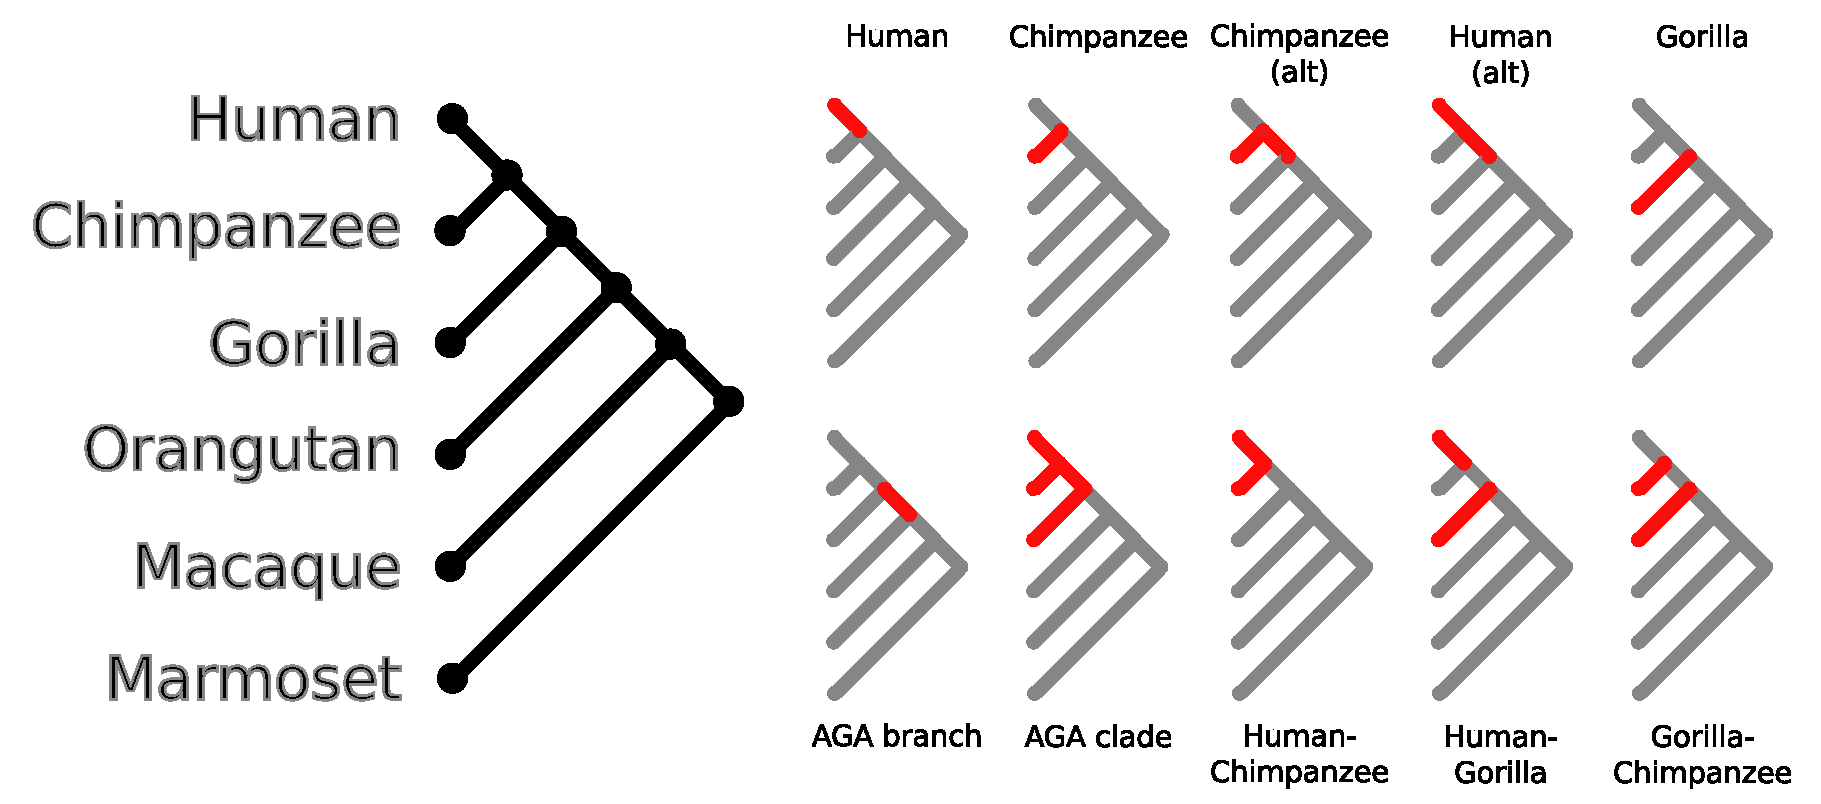
\includegraphics[scale=0.5]{Figs/gorilla_branch_models.pdf}
\caption{Branch models used to construct \ac{lrt} for detecting
  accelerated genes in various branches of the \ac{aga} phylogeny. The
  foreground branches for each model are highlighted in red. The label
  above or below each tree describes which species or group of species
  is under investigation with each model. AGA---African great apes;
  alt.---alternative model.}
\label{fig_gorilla_branch_models}
\end{figure}

To detect signals of accelerated and decelerated evolution in gorilla
and the \ac{aga}, a total of 10 so-called branch models of evolution
were specified. Each branch model separates the phylogenetic tree into
two categories of branches, foreground and background branches, which
are then modeled as evolving with separate \dnds ratios by including
distinct foreground and background \omg parameters in the model
\citep{Yang1998,Yang1998a}. Figure \ref{fig_gorilla_branch_models}
shows the models used in this study, with background branches in gray
and foreground branches in red. Each branch model was designed to
allow for an elevated (accelerated) or decreased (decelerated) \dnds
ratio in a branches of particluar interest to the study of \ac{aga}
evolution. \ac{paml} was used to estimate parameters and calculate the
likelihood value for each model in Figure
\ref{fig_gorilla_branch_models} applied to each coding alignment. A
\ac{lrt} was performed for each model by comparing the likelihood of
the alignment under that branch model to the likelihood of the
alignment under the simpler M0 model, which uses a single \omg
parameter for the entire tree. This test will be referred to as a
branch-LRT to distinguish it from the more commonly used branch-site
LRT described below. The branch-LRT statistic represents the strength
of evidence that a given branch model is a better fit than the simpler
M0 model to a given alignment; in other words, a large statistic can
be interpreted as an indication that the evolution of the gene is
well-explained by different \dnds ratios in the foreground and
background branches of the tree. The \ac{ml} estimate of the two \omg
parameters could be used to identify genes where the estimated
foreground \omg was higher or lower than the background. Genes where
the foreground \omg was higher than the background were categorized as
accelerations, and genes where the foreground \omg was lower than the
background were categorized as decelerations. Using the \ac{lrt}
statistic and the distinction between accelerations and decelerations,
a signed \ac{lrt} statistic was constructed for each branch-LRT, where
accelerated genes were assigned the branch-LRT statistic and
decelerated genes were assigned the negative of the branch-LRT
statistic. In this way, a single number was used to encapsulate the
direction and strength of evidence in support of a shifted \dnds ratio
in the foreground branch of each model presented in Figure
\ref{fig_gorilla_branch_models}.

A highly positive signed branch-LRT score represented strong evidence
for a lineage-specific elevated \dnds ratio. Such an elevated ratio
could be explained either by positive selection or relaxed constraint
\citep{Nielsen2005,Sequencing2005a}. To attempt to distinguish the
former from the latter, we used the branch-site \ac{lrt} implemented
in \ac{paml} \citep{Zhang2005} to identify genes with significant
evidence for positive selection acting along a branch or
clade. Similar to the branch-LRT, the branch-site LRT requires a
predefined separation of branches into foreground and background
categories. However, the branch-site LRT is specifically tuned towards
identifying temporally and spatially localized episodes of positive
selection \citep{Nielsen1998,Yang2002b,Zhang2005}. The branch-site LRT
was run for the Human, Chimpanzee, Gorilla, AGA branch and AGA blade
models shown in Figure \ref{fig_gorilla_branch_models}.

For each model tested, the full length codon alignment was input to
the \texttt{codeml} program from the \ac{paml} package along with a
phylogenetic tree corresponding to the accepted species tree structure
(the labeled tree in Figure \ref{fig_gorilla_branch_models}). The
`cleandata’ option was set to 0 (e.g., alignment columns containing
gaps were not removed from the analysis but were treated as ambiguous
data), and branch lengths inferred by \texttt{codeml} based on the
initial M0 model model analysis were used as the initial branch
lengths for all other models tested.

When the null model of evolution in the branch-LRT is true, the
ac{lrt} statistic---measured as twice the difference in log-likelihood
values between the branch model and the null M0 model---should be
distributed according to a \chisq distribution with one degree of
freedom. The same null distribution was assumed for the branch-site
LRT. Strictly speaking, the branch-site LRT null distribution should
be a 50:50 mixture of a point mass at 0 and \chisq with one degree of
freedom, but the more conservative \chisq distribution is recommended
by Ziheng Yang to guard against violations of model assumptions
\citep{Yang2007}. \pvs for each branch-LRT and branch-site LRT result
were thus calculated by comparing the absolute value of the \ac{lrt}
statistic to a chi-squared distribution with 1 degree of freedom. The
Benjamini-Hochberg method \citep{Benjamini1995} was used to correct
for multiple testing within each branch model by controlling the
\ac{fdr}.

The ``alternative'' models shown in Figure
\ref{fig_gorilla_branch_models}, which were designed to detect
accelerations along the human and chimpanzee lineages while correcting
for the difference in branch length between the human-chimpanzee
terminal branches and the gorilla terminal branch, did not yield
significantly different results from the equivalent uncorrected
models, so results from those tests were discarded from the rest of
the analysis.

\subsection{Branch-LRT and branch-site LRT results}

\begin{table}
\centering \scriptsize
\begin{tabular}{lrrrrrr}
\toprule
 & \multicolumn{2}{c}{Acceleration} & \multicolumn{2}{c}{Deceleration} & \multicolumn{2}{c}{Branch-site LRT} \\
Model / Species & $p<0.05$ & FDR$<0.1$ & $p<0.05$ & FDR$<0.1$ & $p<0.05$ & FDR$<0.1$ \\
  \midrule

\input{Tables/gorilla_lrt_results.txt}
\bottomrule
\end{tabular}
\caption{Branch-LRT and branch-site LRT results. Each row corresponds
  to a model in Figure \ref{fig_gorilla_branch_models}, except for the
  two ``alternative'' models, which were excluded from the
  analysis. Each cell represents the number of genes for which the
  \ac{lrt} was significant at the specified threshold for the given
  model. \pvs were calculated by comparing the \ac{lrt} statistic to a
  \chisq distribution with one degree of freedom. The \acf{fdr} was
  controlled within each model separately for the branch-LRTs and for
  the branch-site LRTs using the \citet{Benjamini1995} method.}
\label{table_gorilla_lrt_results}
\end{table}

Table \ref{table_gorilla_lrt_results} presents for each model, and at
two significance thresholds ($p<0.05$ and LRT$<0.1$), the number of
significantly accelerated and decelerated genes according to the
branch-LRT and the number of positively-selected genes according to
the branch-site LRT. The number of $p<0.05$ accelerated genes for
almost all of the branch models was greater than the expected number
under the null model. Assuming equivalent amounts of acceleration and
deceleration, the expected number of $p<0.05$ accelerations and
decelerations using the branch LRT would be roughly
$11,538\times0.05/2=288$ genes. All models showed an excess of
accelerated genes, with between 300 and 873 genes accelerated at the
nominal $p<0.05$ threshold. Significant evidence for deceleration, was
found at levels equal to or slightly below the null expectation, with
between 151 and 314 decelerations per model. The ``AGA Branch'' model
showed a notable tendency towards lower \dnds ratios, with the fewest
accelerations (300) and most decelerations (314) out of all models
tested.

Looking at strongly accelerated or decelerated genes, defined as those
corresponding to $FDR<0.1$, roughly equivalent numbers were found in
the three terminal lineage models (human / chimpanzee / gorilla) with
between 10-19 strong accelerations and between 1-2 strong
decelerations for each model. The other models were much more
variable, possibly due to differences in power resulting from
different foreground branch lengths, with the AGA Clade model showing
many strongly-shifted genes (56 strong accelerations and 9 strong
decelerations) and the AGA Stem model showing very few (3 strong
accelerations and 1 strong deceleration). The Human-Chimpanzee,
Gorilla-Human, and Gorilla-Chimpanzee models, designed to detect
evidence for parallel accelerations and decelerations, showed roughly
twice as many strongly accelerated and decelerated genes as their
terminal-branch counterparts (29-45 strong accelerations and 3-6
strong decelerations), as might be expected based on the doubled
amount of branch length in the foreground portions of their models.

\section{\acf{go} term enrichments}

Gene ontology (GO) term annotations for the ``biological process''
ontology tree were downloaded from release 60 of the Ensembl human
database \citep{Flicek2011} and assigned to the alignment
corresponding to each human gene. Three complementary methods were
used to assign \pvs for \ac{go} term enrichment among the most
accelerated genes for each branch-LRT performed and genes with
evidence of parallel acceleration in a pair of species. For
lineage-specific accelerations, the 95\% \chisq cutoff value of the
branch-LRT was used to identify accelerated genes. Parallel
accelerations for each species pair were identified by genes with a
minimum branch-LRT value of 1.5 in both species of interest (more
detail on the analysis of parallel accelerations is included in
Section \ref{sec_parallel_accel}).

The first test was a standard one-tailed \ac{fet} applied to the 2x2
contingency table of significant / non-significant genes which were
annotated / not-annotated with a given \ac{go} term. The second
method, implemented in the \topgo program \citep{Alexa2006a}, is also
based on the \ac{fet} statistic but additionally compensates for the
structure of the GO hierarchy by iterating through the directed
acyclic graph and removing nodes from consideration when certain
descendant nodes have already shown significant enrichment (see
\citet{Alexa2006a} for complete details of the algorithm). The main
effect of the \topgo algorithm is to identify and remove semantically
repetitive terms (e.g., terms that are nearby in the \ac{go} ontology
and are annotated with similar sets of genes) from the set of most
significantly enriched results by reducing the \pvs of terms with more
highly-enriched neighboring terms. The third method, implemented in
the \texttt{goseq} program \citep{Young2010a}, accounts for a
potential gene length bias in the propensity for a gene to yield a
significant LRT results. As the sequence length can have a strong
impact on the significance of \ac{lrt} results \citep{Anisimova2001}
and some \ac{go} terms tend to contain longer genes
\citep{Young2010a}, we found it important to correct for this when
identifying enriched terms. The \goseq program first uses the
set of gene-wise \pvs and gene lengths to fit a smoothed \ac{pwf}
which predicts the expected proportion of significant accelerations
given a gene’s length. This \ac{pwf} is then used to adjust the
identification of significantly-enriched \ac{go} terms to correct for
potential over-representation of terms with significantly longer or
shorter mean gene lengths. Although the \goseq program was
designed primarily for the functional analysis of RNA-seq data (where
gene length bias is a widely-acknowledged confounding factor) we found
it to be effective in identifying potentially misleading \ac{go}
enrichment results for the current analysis.

\begin{landscape}
\centering \scriptsize
\begin{longtable}{rrrllrrrrl}
\toprule

Ann. & Sig. & Exp. & ID & Definition & \ac{fet} & \topgo & \goseq &
Len. & Top 5 Significant Genes \\
\endhead

\\
\multicolumn{6}{l}{\normalsize{Table \ref{table_gorilla_go}} (\emph{continued on next page})} & & & & \\
\endfoot

\\[-1.8ex] \hline \hline
\endlastfoot

\midrule
\multicolumn{4}{l}{Human} & & & & & & \\
\midrule
\input{Tables/gorilla_go_1.txt}

\midrule
\multicolumn{4}{l}{Chimpanzee} & & & & & & \\
\midrule
\input{Tables/gorilla_go_2.txt}

\midrule
\multicolumn{4}{l}{Gorilla} & & & & & & \\
\midrule
\input{Tables/gorilla_go_3.txt}

\midrule
\multicolumn{4}{l}{Human-Chimpanzee Parallel} & & & & & & \\
\midrule
\input{Tables/gorilla_go_4.txt}

\midrule
\multicolumn{4}{l}{Gorilla-Chimpanzee Parallel} & & & & & & \\
\midrule
\input{Tables/gorilla_go_5.txt}

\midrule
\multicolumn{4}{l}{Gorilla-Human Parallel} & & & & & & \\
\midrule
\input{Tables/gorilla_go_6.txt}

\midrule
\multicolumn{4}{l}{\ac{aga} Branch} & & & & & & \\
\midrule
\input{Tables/gorilla_go_7.txt}

\midrule
\multicolumn{4}{l}{\ac{aga} Clade} & & & & & & \\
\midrule
\input{Tables/gorilla_go_8.txt}

\bottomrule
\caption{\ac{go} terms enriched for lineage-specific or parallel
  accelerated genes. All terms with \ac{fet} $p<0.05$ are shown sorted
  by their \topgo \pv. Non-significant \pvs from the \topgo
  \citep{Alexa2006a} and \goseq \citep{Young2010a} methods, which
  account for the \ac{go} ontology structure and gene length bias,
  respectively, are shown in gray. The 5 most strongly accelerated
  genes within each category are included for illustrative
  purposes. Ann.---the number of genes annotated with a given term;
  Sig.---the number of significant genes annotated with the term;
  Exp.---the number of significant genes expected given independent
  association between significant genes and \ac{go} terms; Len.---the
  mean length of genes annotated with the term.}
\label{table_gorilla_go}
\end{longtable}
\end{landscape}

The results of the GO enrichment analysis are summarized in Table
\ref{table_gorilla_go}. For each branch model (or pair of species for
parallel accelerations), all terms with a \ac{fet} over-representation
$p<0.05$ and 5 or more significant genes are shown sorted by their
\topgo p-value. Any \topgo or \goseq \pvs above $p=0.05$ are colored
gray instead of black. Terms with non-significant \topgo \pvs are
likely to have a closely-related term with stronger enrichment higher
in the list, while terms with non-significant \goseq \pvs should be
treated with caution due to a detected length bias in the detection of
accelerated genes.

We note that none of the GO term enrichments for any of the tests
remained significant at FDR<0.1 after Benjamini-Hochberg correction
for multiple testing. This indicates that none of the branch model
accelerations were enriched in GO functional categories at a
well-controlled FDR; however, this lack of ontology-wide significance
may be due to a variety of factors including the limited power of
branch models to detect dN/dS shifts, noise in the GO annotation of
genes, or the specific choice of LRT cutoffs in identifying
significant accelerations. Our use of a nominal p<0.05 cutoff for
enriched GO terms yielded a limited set of enriched terms for each
branch model, summarizing the strongest functional associations with
moderately to strongly accelerated genes.

\section{Parallel accelerations}
\label{sec_parallel_accel}
